% !TeX TS-program = pdflatex
\documentclass[xcolor={svgnames,x11names},
%draft
]{beamer}

\usepackage{tikzlings}
\usepackage{tikzducks}
\usetikzlibrary{positioning,shapes}

\setbeamertemplate{navigation symbols}{}
\setbeamertemplate{background canvas}{%
\begin{tikzpicture}[remember picture, overlay]
\node[yshift=1.6cm] at (current page.center){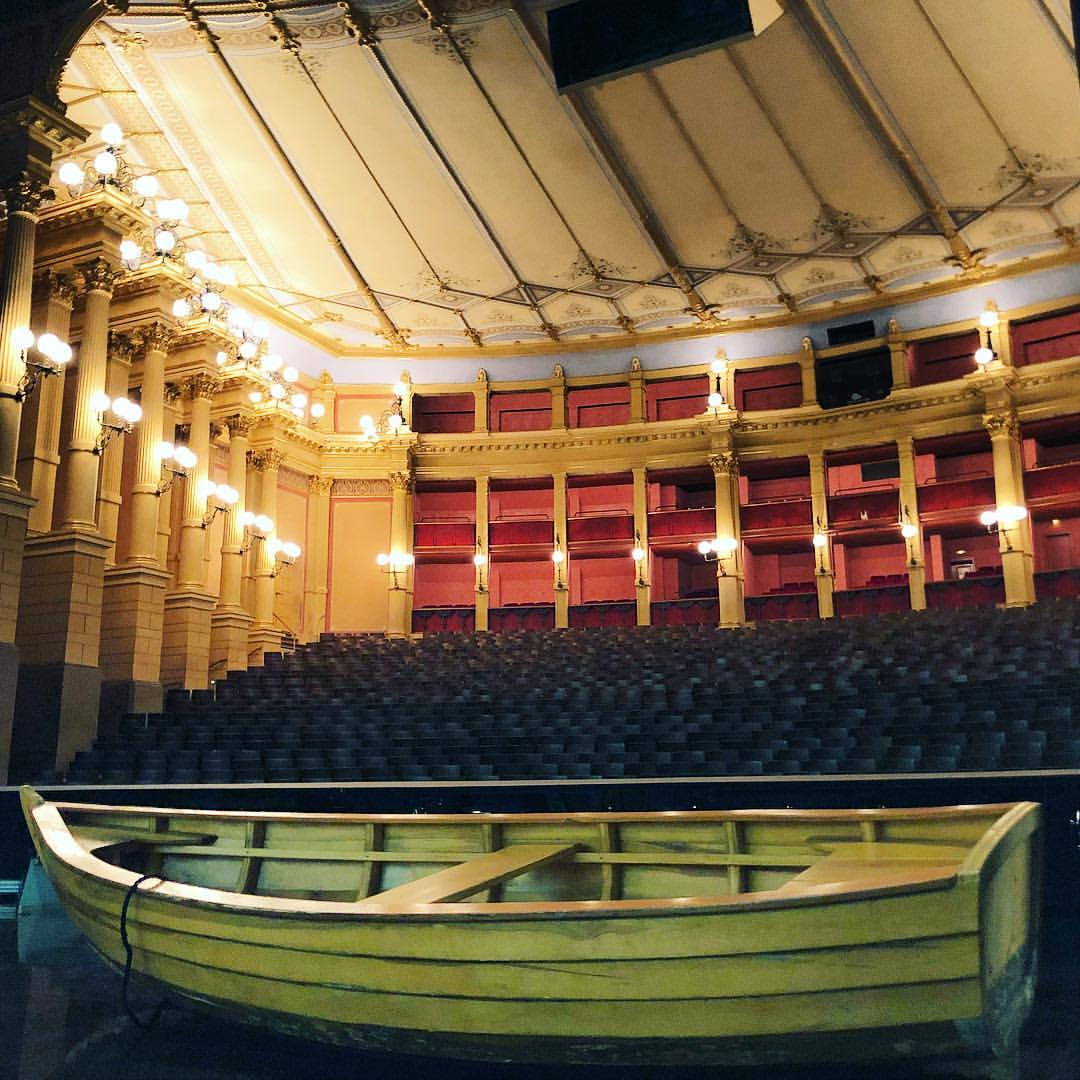
\includegraphics[width=\paperwidth]{Bayreuth}};
% Image credit 
\node[at=(current page.south east),xshift=-6.6cm,yshift=0.2cm]{%
	\tiny\color{white}Image: \url{https://www.instagram.com/p/BmyRNlaFIv3/} \quad Audio: \url{https://commons.wikimedia.org/wiki/File:Sound_Effects_-_Applause_after_a_concert.ogg}
};
\end{tikzpicture}
}

\begin{document}

\begin{frame}
\begin{tikzpicture}[remember picture, overlay]

\node[
	xshift=6cm,
	yshift=-1.5cm+sin(10*\thepage)*cos(10*\thepage)*0.2cm
] at (0,0) {
	
\includegraphics[width=11cm,page=1]{rows}
};
\node[
	xshift=5.75cm,
	yshift=-1.5cm
] at (0,0) {
	
\includegraphics[width=11cm,page=7]{rows}
};
\node[
	xshift=5.5cm,
	yshift=-1.5cm+sin(10*\thepage)*sin(10*\thepage)*0.3cm
] at (0,0) {
	
\includegraphics[width=11cm,page=2]{rows}
};

\node[
	xshift=6cm,
	yshift=-1cm+sin(10*\thepage)*cos(10*\thepage)*0.15cm
] at (0,0) {
	
\includegraphics[width=10.5cm,page=3]{rows}
};
\node[
	xshift=6.25cm,
	yshift=-1cm
] at (0,0) {
	
\includegraphics[width=10.5cm,page=8]{rows}
};
\node[
	xshift=6.5cm,
	yshift=-1cm+sin(10*\thepage)*sin(10*\thepage)*0.25cm
] at (0,0) {
	
\includegraphics[width=10.5cm,page=4]{rows}
};

\node[
	xshift=6.2cm,
	yshift=-0.5cm+sin(10*\thepage)*cos(10*\thepage)*0.12cm
] at (0,0) {
	
\includegraphics[width=10cm,page=5]{rows}
};
\node[
	xshift=6.35cm,
	yshift=-0.5cm
] at (0,0) {
	
\includegraphics[width=10cm,page=9]{rows}
};
\node[
	xshift=6.5cm,
	yshift=-0.5cm+sin(10*\thepage)*sin(10*\thepage)*0.15cm
] at (0,0) {
	
\includegraphics[width=10cm,page=6]{rows}
};

\node[
	xshift=6.8cm,
	yshift=-0.1cm+sin(10*\thepage)*cos(10*\thepage)*0.1cm
] at (0,0) {
	
\includegraphics[width=9.3cm,page=7]{rows}
};
\node[
	xshift=6.65cm,
	yshift=-0.1cm
] at (0,0) {
	
\includegraphics[width=9.3cmm,page=10]{rows}
};
\node[
	xshift=6.5cm,
	yshift=-0.1cm+sin(10*\thepage)*sin(10*\thepage)*0.07cm
] at (0,0) {
	
\includegraphics[width=9.3cm,page=8]{rows}
};

\end{tikzpicture}
\pause[100]
\end{frame}

%\setbeamercolor{background canvas}{bg=}
%\foreach \x in {1,...,100}{
%	\includepdf{cheering-credits.pdf}
%}

\end{document}
